%%%%%%%%%%%%%%%%%%%%%%%%%%%%%%%%%%%%%%%%%%%%%%%%%%%%%%%%%%
%  Copyright (C) 2005 WanT group                         %
%  This file is distributed under the terms of the       %
%  GNU General Public License.                           %
%  See the file `License'  in the root directory of      %
%  the present distribution,                             %
%  or http://www.gnu.org/copyleft/gpl.txt                %
%%%%%%%%%%%%%%%%%%%%%%%%%%%%%%%%%%%%%%%%%%%%%%%%%%%%%%%%%%

\thispagestyle{empty}
\section{How to run \WANT{}: a step by step description}\label{sec:run}

\noindent \underline {NOTE}: At present the \WANT{} code is
implemented to work as a post processing of DFT
calculations done using the codes in: 
\begin{itemize}
  \item[\mydot]  \QUANTUMESPRESSO{} distribution;
  \item[\mydot]  \ABINIT{} package;
  \item[\mydot]  \CRYSTAL{} package;
\end{itemize}

\noindent Following the theoretical description of
Section~\ref{section:intro}, the evaluation of transport
properties requires the following steps:

\begin{itemize}
\item[\mydot] 1. Calculation of DFT electronic structure
\item[\mydot] 2. Calculation of maximally-localized Wannier functions \\
                 (always required except when using CRYSTAL)
\item[\mydot] 3. Calculation of post-processing quantities (DOS, bands, etc)
\item[\mydot] 4. Calculation of quantum conductance.
\end{itemize}


\subsection{DFT Calculations}
\label{subsection:run_dft}
\renewcommand{\theenumi}{\roman{enumi}}
\renewcommand{\labelenumi}{(\theenumi)}
\begin{enumerate}
%
\item Self-consistent calculation using any DFT engine ({\it e.g.} 
      in the \QUANTUMESPRESSO{} or \ABINIT{} distributions). 
      For the description of the input and for further details see 
      the corresponding manuals.
      %
\item Band structure calculation.\\
      \noindent  Starting from the self-consistent charge
      calculated at point $(1)$, compute the eigenstates for a
      {\bf regular {\bf k}-point grid in the complete Brillouin Zone}; the presence of
      the Gamma point is not mandatory. 
      Reduction of \textbf{k}-points due to time-reversal symmetry is being
      investigated but not (yet) allowed. 

      When using \QUANTUMESPRESSO{}, the complete list of
      \textbf{k}-points should be specified in the {\tt K\_POINTS} card.
      It is possible to use the automatic generator, but the flags
      {\tt noinv = .TRUE.} and {\tt nosym = .TRUE.} must be used.
      Otherwise the \textbf{k}-points should be explicitly given. The simple program
      {\tt kgrid.x} in {\tt \~{}want/utility} can be used to generate non-symmetrized
      Monkhorst-Pack grids (run it and follow the instructions).
      
      The {\tt GAMMA\_ONLY} option is also available and fully implemented also in \WANT.
      \\
      If using \QUANTUMESPRESSO{} v3.2 or newer, it is highly recommended to set
      {\tt wf\_collect = .TRUE.} in the {\tt \&CONTROL} namelist (see below). 
      %
\item From \QUANTUMESPRESSO{} to \WANT.\\
      %
      This step is no longer required if setting {\tt wf\_collect = .TRUE.}. 

      \noindent \QUANTUMESPRESSO{} upto v3.1: Use the post processing
      {\tt pw\_export.x} (distributed in the \QUANTUMESPRESSO{} suite\footnote{
      %
      The export utility is already distributed in
      \QUANTUMESPRESSO{} v3.0 (and later versions), but a patch to include it also in 
      versions v2.1.x is available at \WANTURL{}.}),
      %
      to extract the data needed for the following Wannier
      calculations. Data will be stored in the
      newly-created \texttt{\$prefix.export/} directory.  \\
     
      \noindent \QUANTUMESPRESSO{} v3.2 and newer: it is either possible to use the
      {\tt pw\_export.x} utility as before, or just to set 
      {\tt wf\_collect = .TRUE.} in the band-structure calculation. In the latter case, 
      no further run of any post-processing is needed since \WANT{} is able to directly read
      \QUANTUMESPRESSO{} datafiles (stored in the \texttt{\$prefix.save/} directory).

\end{enumerate}


%%%%%%%%%%%%%%%%%%%%%%%%%%%%%%%%%%%%%%%%%%%%%%%%%%%%%%%%%%%%%%
\subsection {Calculation of maximally-localized Wannier
functions}\label{subsection:run_wannier}

Following the list of input parameters as in
Section~\ref{sec:input} (also reported in the {\tt README\_<prog>.input} files
in {\tt \~{}want/docs/}) and the examples in directory {\tt \~{}want/tests/},
create your own input file, that will be used for the following two steps (a-b).
\renewcommand{\theenumi}{\alph{enumi}}
\renewcommand{\labelenumi}{\theenumi)}
%
%
\begin{enumerate}
\item {\tt disentangle.x}: Starting from the data stored at level (iii),
      the code selects the working energy window. From there
      it will extract a selected number ($N$) of WFs to setup the
      Hilbert subspace for Wannier localization.
      For each \textbf{k}-point, the energy window {\bf must}
      contain a number of bands not lower than $N$.
      It is possible to use an inner window (inside the working one) to
      treat frozen-states, for details see Ref.~\cite{ivo2}:
      these frozen Bloch-states will be kept as they are in the Wannier subspace.
      %
      Trial Wannier centers are not mandatory in this step (depending
      on the {\tt subspace\_init} flag).
      To setup these centers, the program {\tt midpoint.x} in 
      {\tt \~{}want/utility } can be used to compute
      the middle points of bonds for a periodic structure (the simple input file 
      is described in the head of the source). 

      {\tt disentangle.x} produces a standard output with the main results,
      and two internal files: {\tt \$prefix\_\$postfix.ovp} and
      {\tt \$prefix\_\$postfix.space} . The former keeps trace of the
      computed overlap and projection integrals (to be re-used in further
      or restarted calculations) while the latter describe the Wannier optimal
      subspace.
      %

\item {\tt wannier.x}: the code reads the same input of {\tt disentangle.x} and
      performs the localization
      procedure leading to the maximally localized WFs.
      The optimal unitary matrices $U(\mathbf{k})$ governing the transformation between
      Bloch and Wannier states are obtained.
      In this step different trial centers can be used, but it is a standard procedure
      to keep those used in the {\tt disentangle.x} run.
      {\tt wannier.x} produces a standard output with describing the iterative
      path to the optimally localized WFs.
      The code also writes two internal data-files: {\tt \$prefix\_\$postfix.wan}
      containing the $U(\mathbf{k})$ and {\tt \$prefix\_\$postfix.ham} with the
      hamiltonian matrix elements on the Wannier basis.
      %
\end{enumerate}
%
%

\noindent
Further physical information may be obtained as external
post-processing of the WFs calculation. They are not necessary for
the transport calculation, but they may be useful for a
better understanding of the intrinsic electronic properties of the
system. These codes require a separate input, to be generated
following Sec.~\ref{sec:input} or the
{\tt \~{}want/docs/README\_<prog>.input} files.

%
%
\begin{itemize}
%
\item {\tt bands.x}: the code computes the interpolated band-structure
      of the system along selected direction in the Brillouin Zone.
      The comparison with independently calculated DFT eigenvalues is
      a nice test to check the localization of the obtained WFs.
      When they are well behaved ({\it i.e.} localized), only few $\mathbf{R}$ lattice
      vectors are required to described the Hamiltonian on the Wannier basis
      [$H_{ij}(\mathbf{R})$]
      Starting with a small set of $\mathbf{k}$ in the DFT calculation
      we obtain the Hamiltonian on the related (small) set of lattice vectors.
      When WFs are well localized
      the Hamiltonian is fully described on this set of $\mathbf{R}$ and we can
      diagonalize it for an arbitrary large set of $\mathbf{k}$ points
      (as a post-processing of the Wannier code). This is the
      interpolation of the band structure using WFs. If they are not localized
      we are essentially throwing away some non-negligible matrix elements
      in the Hamiltonian representation, and the bands
      are not accurate. Typical unphysical oscillations appears in these cases.
      %

\item {\tt dos.x}: the code computes the {\it density of states} (DOS) 
      of the system interpolating the band structure by means of WFs, as
      for {\tt bands.x}. Since the DOS is a quantity integrated (or better summed)
      over the BZ, a uniform mesh of $\mathbf{k}$ points (supplied by the user)
      is adopted.
      Once a self-consistent calculation is performed (and WFs computed), this code can be 
      used to obtain accurate DOS. 
      %

\item {\tt plot.x}: this is an utility to plot WFs in real space.
      The plotting region can be tuned and a generic number of WFs can be
      handled in a single run.
      The real or imaginary parts of the WFs as well as their squared moduli are
      allowed fields to be plotted.
      The code produces plot files in various formats (txt, gaussian cube, xsf, plt)
      allowing the use of standard open source visualization-packages
      such as gOpenMol or xCrysDen. Output files are labelled as
      {\tt \$prefix\_\$postfix\_WF\$type\_\$num.\$fmt}, where {\tt \$type} can be
      {\tt R, I, M} according to the plotted field (real or imaginary part, squared
      modulus), {\tt \$num} is the index of the chosen WF and {\tt \$fmt} is the
      output format. If needed, an auxiliary file with the atomic structure
      in the {\tt xyz} format is also produced.
      %
\item {\tt blc2wan.x}: transforms a generic (eventually dynamic) operator
      given on the Bloch eigenstates basis $A_{mn}(\mathbf{k}) =
      \langle \psi_{m\mathbf{k}} |\, \widehat{A}(\omega) \,|
      \psi_{n\mathbf{k}} \rangle$ to the WFs representation.
      Using the unitary matrices $U(\mathbf{k})$ calculated during the Wannier localization
      (b) and the definition of the Wannier subspace in terms of the Bloch eigenstates
      (a), $\widehat{A}(\omega)$ is described in terms of the matrix elements
      $A_{ij}(\mathbf{R}) = \langle w_{i\mathbf{0}} |\, \widehat{A}(\omega) \,|
      w_{j\mathbf{R}} \rangle$ .
\end{itemize}

%%%%%%%%%%%%%%%%%%%%%%%%%%%%%%%%%%%%%%%%%%%%%%%%%%%%%%%%%%%%%%%

\subsection {Calculation of electronic transport}
\label{subsection:transport}

Using the hamiltonian matrices calculated in step (b) we can
calculate both the {\em bulk} and the {\em two-terminal}
transmittance. Input file may be generated following
Sec.~\ref{sec:input} or the {\tt README\_<prog>.input} files in {\tt
\~{}want/docs}. The main result of the calculation is the quantum
transmittance across the conductor region.
Conductance is given in $2e^2/h$ units.
Calculations are performed using the Fisher-Lee formula according
to Sec.~\ref{subsec:tran}. As an auxiliary piece of information,
the density of states (DOS) projected on the conductor is also
written. This DOS is computed as the
trace of the conductor Green's function $ N(E) = -(1/\pi)\,
\text{Im} \, \text{Tr}\, G_C(E)$.

Except the special case of the bulk transmittance (see below), the systems one is
interested in are generally not periodic along the transport direction. This does not
in principle avoid a 2D periodicity in the orthogonal plane. The use of
2D mesh of $\mathbf{k}$-points in this context is implemented in the present
version of the code.  \\

Note also that \texttt{conductor.x} has been parallelized over the 
main frequency loop, and therefore turns out to be very scalable.
To compile this part of the code using a parallel environment, configure
with the command:

\texttt{ ./configure --enable-parallel [other-options]}

\noindent
according to Sec.~\ref{section:install}. 


%%%%%%%%%%%%%%%%%%%%%%%%%%%%%%%%%%%%%%%%%
%
%
\begin{figure}
   \centering
   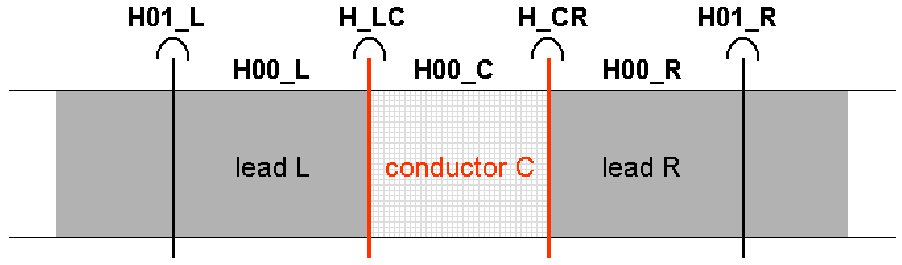
\includegraphics[clip,width=0.6\textwidth]{lcr}
   \caption{Schematic definitions for Hamiltonian block matrices used in
            transport calculations. \label{fig:matrix_naming}}
\end{figure}
%
%
\noindent Before discussing in more detail the actual calculations
performed by the transport code, we precisely define the adopted
convention for the names of the real-space ({\i.e.} WF)
Hamiltonian blocks. Given a conductor (C) connected to left (L)
and right (R) leads, containing respectively $N_C$, $N_L$ and
$N_R$ WFs,
we define the following matrices (see Fig.~\ref{fig:matrix_naming}): \\

%
%
\begin{table}[h]
%
\begin{tabular}{lllll}
\texttt{H00\_L} &=& $N_L\times N_L$ on-site hamiltonian
of the leads L & (from L-bulk calc.)\\
\texttt{H01\_L} &=& $N_L\times N_L$ hopping hamiltonian
of the leads L & (from L-bulk calc.) \\
\texttt{H00\_R} &=& $N_R\times N_R$ on site hamiltonian
of the leads R & (from R-bulk calc.) \\
\texttt{H01\_R} &=& $N_R\times N_R$ hopping hamiltonian
of the leads R & (from R-bulk calc.) \\
\texttt{H00\_C} &=& $N_C\times N_C$ on site hamiltonian
of the conductor C & (from C-supercell calc.) \\
\texttt{H\_LC}  &=& $N_L\times N_C$ coupling
between lead L and conductor C & (from C-supercell calc.) \\
\texttt{H\_CR}  &=& $N_C\times N_R$ coupling
between conductor C and lead R & (from C-supercell calc.)
%
%
\end{tabular} \\
%
\caption {Main Hamiltonian blocks needed for transport calculation
          \label{tab:hamiltonian_blocks} }
\end{table}
%
%
%
\noindent In the general case we need to compute the electronic
structure and WFs for three different regions L, C, R. Very often
one is interested in a situation where the leads are composed of
the same material. We will discuss in more detail this case, the
being treatable in the same way except for a more complicated
geometry in the conductor region.

First we note that the conductor calculation should contain part
of the leads in the simulation cell, in order to treat the
interface from first principles. The amount of lead layers to be
included should be converged up to the local electronic structure
of the bulk lead is reached at the edges of the supercell. This
convergence can be controlled taking a look at the hamiltonian
matrix elements on Wannier states located in the lead region ({\it
e.g.} nearest neighbor interactions). Note that this is a physical
condition related to the need for a matching of different
calculations and not to the peculiar use of WFs as a basis:
nevertheless the smaller the WFs the more independent on the
environment are the matrix elements, leading to a faster
convergence.

As from Tab.~\ref{tab:hamiltonian_blocks}, the {\tt H00\_C} term
can be obtained directly from the conductor supercell calculation.
The on-site block ($\mathbf{R}=\mathbf{0}$) is automatically
selected. The same is true in general for the lead-conductor
coupling (consider for instance {\tt H\_CR}): here the rows of the
matrix are related to (all) the WFs in the conductor reference
cell while the columns usually refer to the some of them in the
nearest neighbor cell along transport direction (say {\it e.g.}
the third lattice vector). The {\tt H\_CR} Hamiltonian we are
interested in is therefore a $N_C \times N_R$ submatrix of the
$\mathbf{R}=(0,0,1)$ block. In order to understand which rows and
columns should enter the submatrix, we need to identify some WFs
in the conductor with those obtained for bulk lead calculation.
This assumption is strictly correlated with that about the local
electronic structure at the edge of the conductor supercell: the
more we reach the electronics of the leads, the more WFs will be
similar to those of bulk leads. As before, the smaller the WFs,
the more independent of the environment they are. In this way we
can extract the lead-conductor coupling matrices directly from the
supercell conductor calculation. Much care must be taken in this
step in order to avoid numerical noise. See Sec.~\ref{sec:input}
for the input file details.

The missing Hamiltonians ({\tt H00\_x, H01\_x}, where {\tt x=L,R})
can be obtained from direct calculations for the bulk leads and
are taken from the $\mathbf{R}=(0,0,0)$ and $\mathbf{R}=(0,0,1)$
blocks respectively (as from Tab.~\ref{tab:hamiltonian_blocks}).
All these Hamiltonian matrix elements are related to a zero of the
energy scale set at the Fermi energy of the computed system (the
top of valence band for semiconductors). It is not therefore
guaranteed the zero of the energy to be exactly the same when
moving from the conductor to the leads (which comes from different
calculations). In order to match the hamiltonian matrices at the
boundary, it is necessary to check that the corresponding diagonal
elements (the only affected by a shift in the energy scale) of
{\tt H00\_L, H00\_C and H00\_R} matrices are aligned (see the end
of the {\tt wannier.x} output-file to easily find these elements).
If not, a rigid shift may be applied.

Alternatively, the {\tt H00\_x} and {\tt H01\_x} matrices may be
obtained from the conductor supercell calculation too. We need to
identify the WFs corresponding to some principal layer of the
leads and extract the corresponding rows and columns. This
procedure is not affected by any energy-offset problem, but larger
supercells should be used in order to obtain environment
(conductor) independent matrices. See the tests to check the
numerical performance of these schemes.
%
\\

\noindent The transport code distributed within the \WANT{} package is
{\tt conductor.x} which calculates both the
{\em bulk} and the {\em two-terminal} transmittance for the systems.
While in the former case we
only need the {\tt H00\_C} and the {\tt H\_CR} matrices, the whole complexity
of input data described above is managed in the latter.
